\documentclass[conf]{new-aiaa}
%\documentclass[journal]{new-aiaa} for journal papers
\usepackage[utf8]{inputenc}

\usepackage{graphicx}
\usepackage{amsmath}
\usepackage[version=4]{mhchem}
\usepackage{siunitx}
\usepackage{longtable,tabularx}
\setlength\LTleft{0pt} 

\title{Homework 6: Nuclear Propulsion}
\author{Riley J. Kyle} 

\begin{document}

\maketitle


\begin{figure}[hbt!]
    \centering
    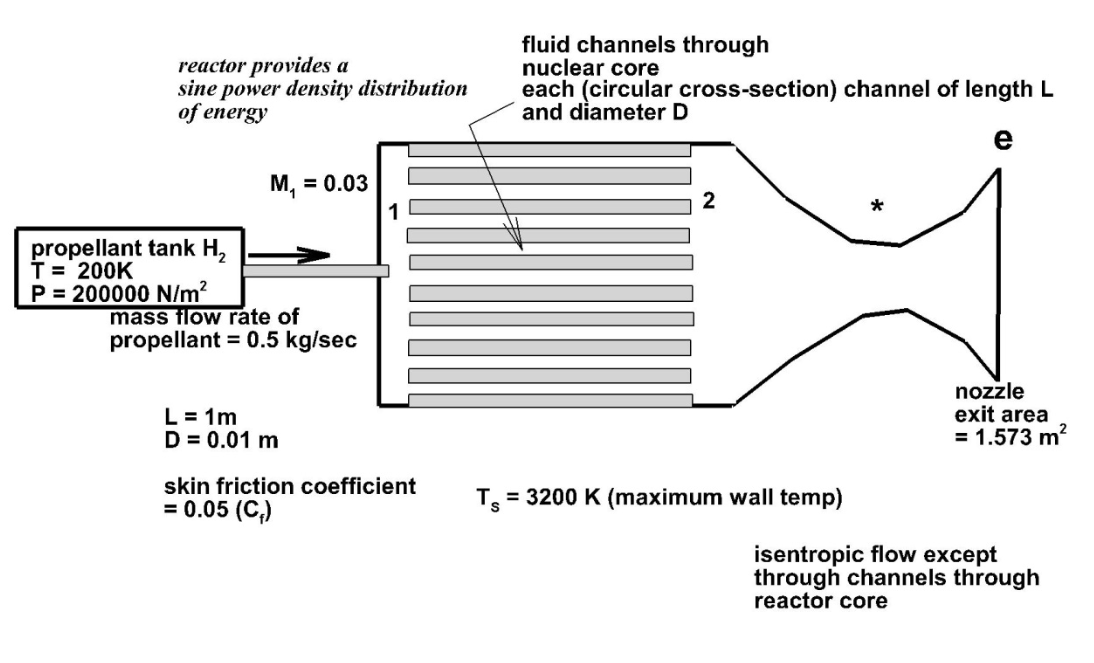
\includegraphics[width=1\textwidth]{engine_diag.png}
\end{figure}

\textbf{Answers:}   \newline \newline
$x_{T_{max}} = $    \newline \newline
$Q\dot = $          \newline \newline
$F = $              \newline \newline
$I_{sp} = $         \newline \newline

\clearpage
Conditions for sin power density distribution.\newline
\begin{enumerate}
    \item zero slope of $T_t$ at $x=0$

    \item max slope of $T_t$ at $x=L/2$

    \item zero slope of $T_t$ at $x=L$
\end{enumerate}


Additionally $T_s\rightarrow T_w$ occurs at some $x$ between $x=L/2$ and $x=L$.


\begin{equation}
    \label{sample:equation}
    \sum^{n}_{i=1}{2n-1}
\end{equation}


\end{document}
